\documentclass[dvipdfmx]{jsarticle}
\usepackage[dvipdfmx]{graphicx}
\usepackage{amsmath, amssymb}
\usepackage{url}
\usepackage{mathtools}
\usepackage{here}
\begin{document}
\title{週間進捗報告}
\author{権藤陸}
\date{2022年4月27日}
\maketitle
\section{進捗}
指定の論文[1]を結論まで読んだ。

\section{手法}
胎児心拍数(FHR: Fetal Heart Rate)の推定精度を改善するためのアルゴリズムは、2段階に分けることができる。1段階目は、未フィルタリングFHR推定値と、分類された胎児のSQIを入力として、シングルチャネルHR推定である。2段階目は、マルチチャネルデータフュージョンであり、これは、各チャネルのカルマンフィルタによるFHR推定値と胎児のSQI, KFアルゴリズムの副産物としての信号を使用するものである。

提案法の性能指標としては、Cohenの$\kappa$係数、Krippendorffの係数、およびFHR推定値とアノテーションされたFHR値の二乗平均平方根誤差(RMSE: Root Mean Squared Error)が用いられている。

\begin{itemize}
    \item ARモデル

    時系列モデルの一つ。自己回帰モデルとも呼ばれる。現在の値を過去のデータを用いて回帰するモデルで、経済指標予測や気象予測等の時系列データの予測に最も一般的に用いられる方法である。今回論文で出てきた1次ARモデルは、$y_t = \phi_0 + \phi_1 y_{t-1} +\epsilon_t$の形で表され、$\phi_0, \phi_1$は最小二乗法で求められる回帰係数、$y_{t}, y_{t-1}$はそれぞれ時刻$t, t-1$におけるデータ、$\epsilon_t$は攪乱項で平均0、分散$\sigma^2$のノイズである。
    \item 累積分布関数

    連続確率変数$X$の累積分布関数は、確率密度関数の積分として表すことができ、
    \begin{equation}
    f(x) = F_X (x) = \int_{-\infty}^x f_X (t) dt
    \end{equation}
    と表される。
    \item グリッドサーチ

    モデルのハイパーパラメータを探索する手法。全パラメータの組み合わせを試し、最も高い精度が出るパラメータを見つける。全組み合わせを網羅的に探索するため、求めるパラメータを発見できる確実性がある反面、計算時間がかかるという欠点がある。
    \item 交差検証(クロスバリデーション)
    
    主にモデルの汎化性能を測る目的で行われる。K-分割交差検証は、データをK個に分割し、1つをテストデータに、残りのK-1個を学習データとすることで正解率の評価を行う。データ全てが1度ずつテストデータになるようにK回学習を繰り返し、精度の平均をとる手法である。
\end{itemize}
\section{結果}
単純ベイズ分類器を用いた5クラスへの分類精度は、平均で$\kappa = 0.44 \pm 0.03(筆者はmoderateと評価)、\alpha = 0.65 \pm 0.04(good)$であった。
カルマンフィルタ適用前後のシングルチャネルFHRの結果とマルチチャネルの結果は図1のように示される。

\begin{figure}[htbp]
\begin{center}
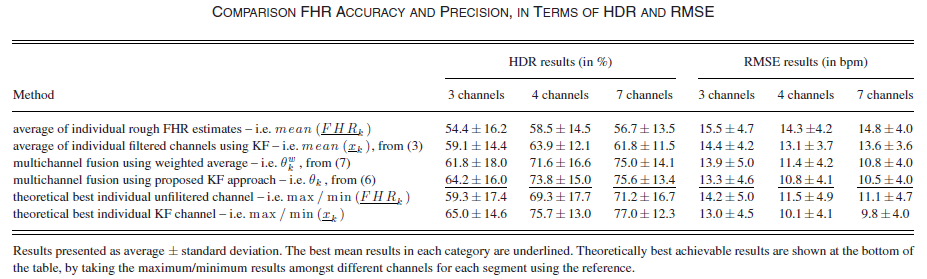
\includegraphics[width=
0.95\linewidth]{./paper/FHR_table.png}
\end{center}
\caption{HDRとRMSEによるFHRの精度の比較}
\end{figure}

\section{議論点}
\begin{itemize}
    \item 今回使用したデータセットは文献上のFHR解析のためのほとんどのデータセットよりもサイズが大きいにもかかわらず、多くのデータの信号品質が悪いか低いものであった。
    \item  学習データには、胎児や母体の不整脈と異所性拍動の出現数が非常に少なかったために、提案した分類法の臨床への適用が制限される。

    $\rightarrow$ より大規模なデータセットの収集が必要
    \item 著者らがSNRや信号品質について評価し、アノテーションする際に定義したコンセンサスはあくまで主観的な概念であった。
    \item 本研究で用いられたデータセグメントの長さは5秒であったが、いくつかのSQIアルゴリズムにとってはより長いセグメントの方が適している。しかし、提案アルゴリズムのウィンドウの長さとオンライン機能の間にはトレードオフの関係があることを考慮すれば適切な長さであったと言える。
    また、SQIインデックスを拡張し、1拍単位で適用することに焦点を当てた研究を行う必要がある。
    \item ほとんどの誤分類は、隣接するクラス内にあり、5つのクラスに分類していたものを「許容」・「許容できない」の2グループに分類し直すことで、精度92.1\%、感度49.3\%、positive predictive value = 87.8\%を達成した。感度が低いのは、質の高い信号の数が著しく少ないためと考えられる。
    \item 質の高い信号が少ないというアンバランスさを考慮すると、利用可能な9065セグメントに対して、使用したデータセットの次元数"45"が分類タスクに不利な影響を与える可能性がある。この問題には、特徴選択を適用して次元を削減することで、分類器の性能を向上させることができれば改善される可能性がある。
    \item カルマンフィルタを用いたFHRのマルチチャネル推定は、HDR(Heartbeat Detection Rate)とRMSEの両面で最良の性能を示した。カルマンフィルタの性能は、誘導線の数が増加するにつれて単調に増加していることから、うまく付加的な情報を取り込めていると考えられる。
\end{itemize}

\section{結論}
複数の胎児SQIメトリクスを調査し、5秒セグメントにおける胎児信号の品質を推定するための単純ベイズ分類器に適用した。この分類器をカルマンフィルタアルゴリズムと組み合わせて使用し、マルチチャネルの非侵襲的な胎児の心電図記録からオンラインFHR推定を改善した。
\section{疑問}
\begin{itemize}
    \item "online approach"の意味について
\end{itemize}
\section{計画}
発表に向けて細かい読み込み・プレゼン制作
\begin{thebibliography}{}
\item Fernando Andreotti, Felix Graser, Hagen Malberg, and Sebastian Zaunseder. Non-invasive Fetal ECG Signal Quality Assessment for Multichannel Heart Rate Estimation. IEEE TRANSACTIONS ON BIOMEDICAL ENGINEERING. 2017, vol. 64, no. 12, p. 2793-2802.
\end{thebibliography}
\end{document}